\chapter{Vers une amélioration possible du support exécutif à travers la simulation}\label{chap:simulation}
\chaptertoc

\begin{todo}
  graphe récapitulatif avec interactions
\end{todo}

Le chapitre~\ref{chap:contrib:characterization} a montré qu'il était possible de caractériser précisément à la fois les machines et les parties critiques d'application vis à vis de ces machines.
Cela a pu confirmer et chiffrer l'importance de la localité des données sur les architectures NUMA.
Le chapitre~\ref{chap:contrib:openmp} a montré comment il était possible d'étendre un modèle de programmation et les supports exécutifs pour mieux prendre en compte la localité des données, et globalement améliorer l'ordonnancement de l'application.

À partir de là, certaines questions peuvent se poser~:
\begin{itemize}
  \item Compte tenu des caractéristiques de l'application et des machines, peut on faire mieux ? Et si oui~:
  \item Quelle marge reste-t'il à gagner par rapport aux ordonnancements théoriques connus ?
  \item Quelles caractéristiques faudrait il prendre en compte ?
\end{itemize}

Le coût en temps d'un développement de nouvelles analyses ou stratégies dans les compilateurs et supports exécutifs peut être important. Ainsi avant de se lancer il serait préférable de connaître le potentiel des améliorations.
Nous avons donc développé un simulateur, dans le but de pouvoir apporter une réponse aux questions ci-dessus, sans pour autant impliquer de lourds développements logiciel.

Ce chapitre est organisé de la façon suivante~: la section~\ref{sec:simulation:archi} décrit l'architecture générale du simulateur.
La section~\ref{sec:simulation:modeles} fait un point sur les différents modèles envisagés, et la section~\ref{sec:simulation:resultats} montre des résultats préliminaires obtenus avec ces modèles, en apportant des premières pistes de réponses aux questions posées.
Enfin la section~\ref{sec:simulation:next} décrit quels améliorations du simulateur seraient possible pour améliorer son réalisme.

\begin{todo}
TODO rajouter introduction section Julien si possible
\end{todo}


\section{Fonctionnement du simulateur}\label{sec:simulation:archi}

Le simulateur implémente un certain nombre de concepts que nous avons déjà abordés, détaillés ci-après.


\paragraph{Données~:} elles sont représentés comme des blocs de tailles fixes, qui sont associés à un cœur lors de leur création (pour simuler la politique \emph{first-touch} du système d'exploitation).

\paragraph{Tâches~:} elles sont représentées de manière similaire à ce qui se fait dans les supports exécutifs.
Chaque tâche est composée d'une série d'actions séquentielles, pouvant être de trois types différents~:
\begin{itemize}
  \item \emph{READ}~: lecture d'un bloc de données
  \item \emph{WRITE}~: écriture d'un bloc de données
  \item \emph{COMPUTE}~: calcul avec un certain nombre d'instructions.
\end{itemize}

De plus des dépendances entre tâches peuvent être ajoutées en attachant un ensemble de prédécesseurs à une tâche donnée.

\paragraph{Topologie~:}
De manière similaire à ce que nous avons utilisé lors de nos travaux, nous avons considéré ici deux niveaux de hiérarchie, avec une file de tâche prêtes par cœur, et une file de tâche prêtes par nœud.

\paragraph{Ordonnancement~:}
L'objectif était de simuler le comportement d'un support exécutif similaire à ceux que nous avons utilisé dans le chapitre~\ref{chap:contrib:openmp}, nous avons donc basé l'ordonnancement au sein du simulateur sur du vol de travail.
Le moteur d'exécution repose sur deux fonction \emph{steal} et \emph{push}, devant implémenter les processus de vol et de placement d'une tâche, respectivement.
Pour le besoin des premières comparaisons, nous avons implémenté deux heuristiques différentes, similaires à celles utilisées dans les résultats de la section~\ref{sec:contribs:perf_eval}~:
\begin{itemize}
  \item \emph{RandLoc}~: elle effectue du vol de travail aléatoire de base et un placement des tâches prêtes localement~; elle est équivalente à la combinaison de stratégies \emph{sRand/pLoc} décrites dans la section~\ref{sec:openmp:runtime:select}.
  \item \emph{Affinity}~: elle effectue un vol de travail hiérarchique et un placement des tâches conformément à l'affinité des données~; elle est équivalente à la combinaison \emph{sNumaProc/pNumaWLoc} décrites dans la section~\ref{sec:openmp:runtime:select}.
\end{itemize}


\paragraph{Modèle~:}
Un modèle fourni des informations cruciales~: il défini la topologie de la machine (nombre de cœurs, de nœuds, ainsi que les associations cœur/nœud), il défini également le coût de chaque opération (exprimé en secondes) en fonction de son type et du type de la tâche effectuant l'opération.


\section{Modèles envisagés}\label{sec:simulation:modeles}

Nous avons choisi de commencer à étudier l'application qui nous a servi de cas d'étude pour le chapitre~\ref{chap:contrib:characterization}~: Cholesky.
Les données récoltées à l'aide de \outil nous ont permises de comprendre précisément le comportement de chacun des quatre noyaux impliqués dans la factorisation de Cholesky.
Nous avons donc implémenté un Cholesky similaire dans le simulateur, et défini plusieurs modèles afin d'évaluer le simulateur et éventuellement les bornes de l'application en terme de performances.

Comme les données récoltées sur les noyaux incluent la totalité des actions des tâches (lecture, calcul, et écriture), nous avons donc dans un premier temps utilisé un modèle simplifié, où la quantité de données en lecture et écriture est ignorée, mais ou la partie \emph{COMPUTE} inclue ces accès, et dépend du placement du bloc de données sur la machine simulée.

\begin{table}[t!]
\def\arraystretch{1.5}
\centering
\begin{tabular}{|c||c|c|c|}\hline
  \multirow{2}{*}{Noyau} & \multirow{2}{*}{\makecell{Nombre d'exécution concurrentes\\(threads)}} & \multicolumn{2}{c|}{Performance (GFLOPS)} \\ \cline{3-4}
    & & Données locales & Données distantes \\ \hline
  \multirow{2}{*}{\potrf}
    & 1 & 11.48 & 11.66 \\ \cline{2-4}
    & 192 & 9.30 & 8.81 \\ \cline{2-4}
  \hline
  \multirow{2}{*}{\gemm}
    & 1 & 16.92 & 17.10 \\ \cline{2-4}
    & 192 & 14.45 & 12.82 \\ \cline{2-4}
  \hline
\end{tabular}
\caption{Tableau illustrant les performances (en GFLOPS) de certains noyaux sur des matrices de taille 512, sur idchire}\label{tab:simu:perf-kernels-idchire}
\end{table}

Afin de pouvoir illustrer les différents modèle que nous avons testés, le tableau~\ref{tab:simu:perf-kernels-idchire} regroupe quelques exemples de performance pour certains noyaux, pour une taille de matrice de 512, en fonction de la charge de la machine (comme décrit dans la section~\ref{sec:contribs:apps:cholesky:scenario}) et du type d'accès.

Cet extrait de performances permet de montrer que si la localité des données n'a pas d'impact positif pour un unique thread, en pleine charge la différence de performance est significative.

Nous avons donc dégagé plusieurs modèles, décrit ci-dessous.

\paragraph{Modèle "Minimum"~:} ce modèle a pour but d'estimer la performance minimum que l'on est en droit d'attendre d'un support exécutif implémentant une stratégie de vol de travail naïve.
Pour se faire, nous avons considéré seulement les performances minimales de chacun des noyaux pour le coût de chaque tâche (il est généralement atteint pour une charge équivalente au maximum de cœur, avec des accès aux données distants), et ceci quelque soit le vrai type d'accès au cours de la simulation.

\paragraph{Modèle "Maximum"~:} à l'inverse l'objectif de ce modèle est de donner une borne supérieure pour les performances du support exécutif.
Nous avons donc considéré seulement les performances maximales de chacun des noyaux pour le coût de chaque tâche, et ceci quelque soit le vrai type d'accès au cours de la simulation.

\paragraph{Modèle "Affinity"~:} l'objectif de ce modèle est d'essayer de simuler au plus près le comportement des noyaux.
La simulation étant lancée sur un nombre de cœurs connus, nous avons chargé les performances de référence des noyaux correspondant à la charge de la machine simulée.
Lors de la simulation nous déterminons si les accès en écriture de la tâche sont locaux ou distant, et le coût de la tâche correspondante est utilisé.




\section{Résultats préliminaires}\label{sec:simulation:resultats}


Nous avons commencé par comparer les modèles entre eux.
Pour ce faire nous avons choisi un cas réel ou l'affinité avait un impact significatif~: une taille de bloc de 512 pour une taille de matrice de 32768, avec des blocs de données répartis de manière cyclique sur la machine.
Les résultats des simulations avec les différents modèles sont montrés sur la figure~\ref{fig:simu:modeles:idchire}.

\begin{figure}[h!]
  \centering
  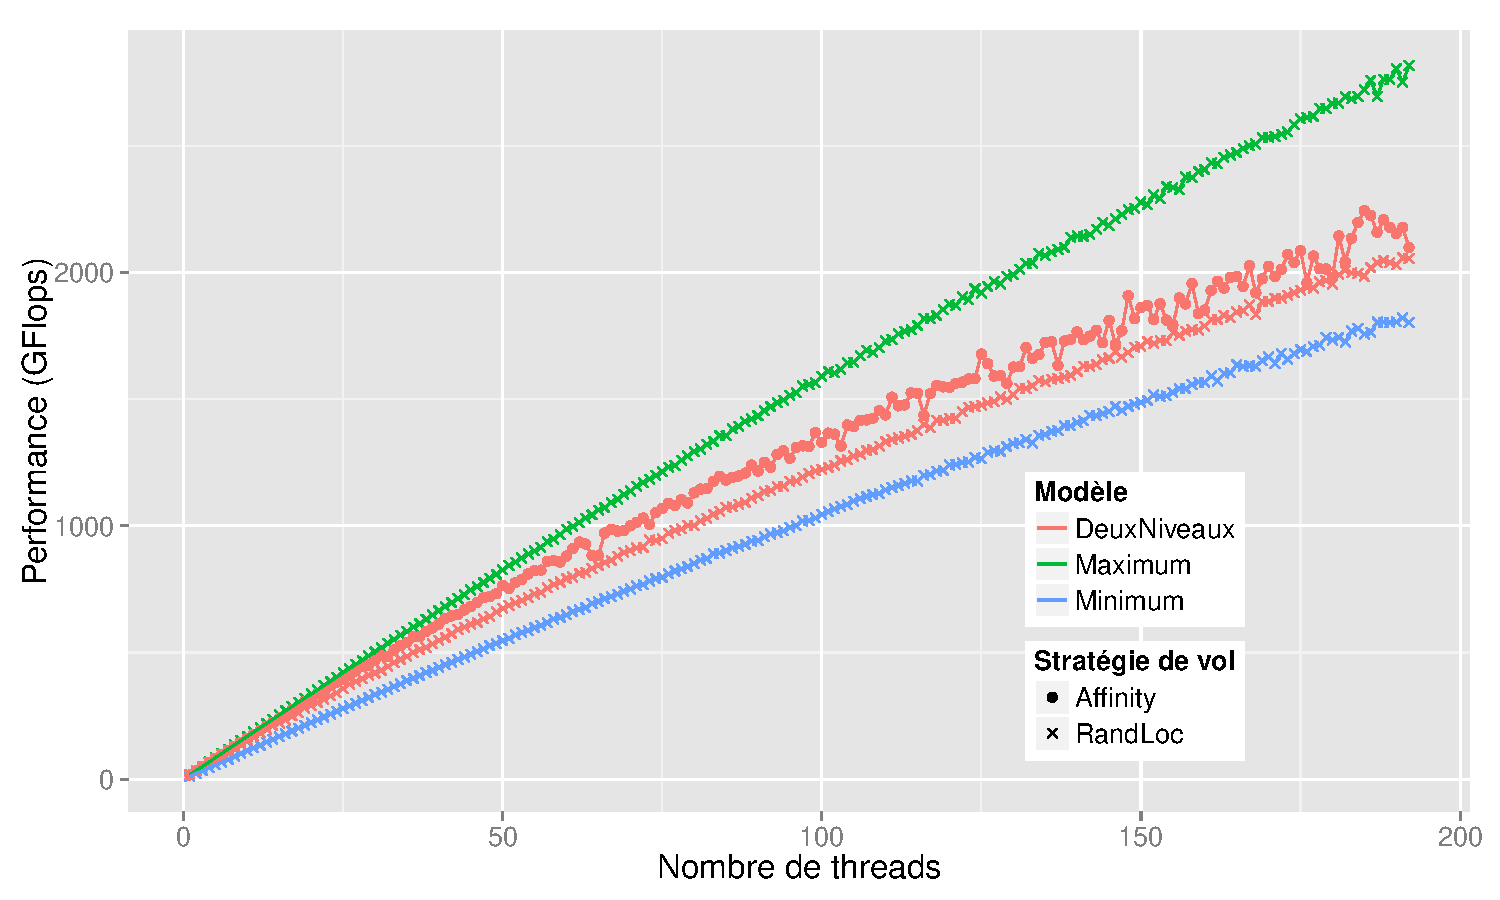
\includegraphics[width=\textwidth]{simu_min_max_affinity_idchire}
  \caption{Comparaison des différents modèles et stratégies, basés sur les références d'idchire. Taille de bloc~: 512, taille de matrice~: 32768}\label{fig:simu:modeles:idchire}
\end{figure}


Les premières observations à faire sur cette figure sont plutôt positives~: les performances affichées semblent réalistes, le modèle \emph{Affinity} est correctement encadré par les modèles \emph{Minimum} et \emph{Maximum}, et au sein du modèle \emph{Affinity}, il y a bien une différence claire entre un vol de travail <<naïf>> --- \emph{RandLoc} --- et un vol de travail hiérarchique et sensible à l'affinité --- \emph{Affinity}.

\begin{table}[h!]
\def\arraystretch{1.5}
\centering
\begin{tabular}{|c||c|c|c|c|}\hline
  \multirow{2}{*}{Stratégie} & \multicolumn{2}{c|}{Lectures} & \multicolumn{2}{c|}{Écritures} \\ \cline{2-5}
    & Locales & Distantes & Locales & Distantes \\
  \hline
  \emph{RandLoc} & 4 380 & 117 066 & 1902 & 43 858 \\
  \hline
  \emph{Affinity} & 15 343 & 88 045 & 22 556 & 23 204 \\
  \hline
\end{tabular}
\caption{Nombre de lectures et écritures de blocs locaux ou distants en fonction de la stratégie de vol}\label{tab:simu:acces-blocs-idchire}
\end{table}
\begin{todo}
Note : cumul des lectures dans la table différent puisque cache infini : si lecture une fois sur le nœud, c'est gratos après si la version change pas.
\end{todo}

Cela est confirmé en regardant le nombre de lectures et écritures locales ou distantes, rapportées dans le tableau~\ref{tab:simu:acces-blocs-idchire}.
Ce tableau montre que le nombre d'accès distants est significativement diminué par l'utilisation d'une stratégie de vol de travail sensible à l'affinité~: le nombre d'écritures distantes est réduit de moitié, tandis que le nombre de lectures distantes est réduit d'environ 25\%.


Ces figures sont bien sur issues de simulation~; que valent elles en comparaison aux chiffres obtenus à travers les expériences ?

\begin{figure}[t!]
  \centering
  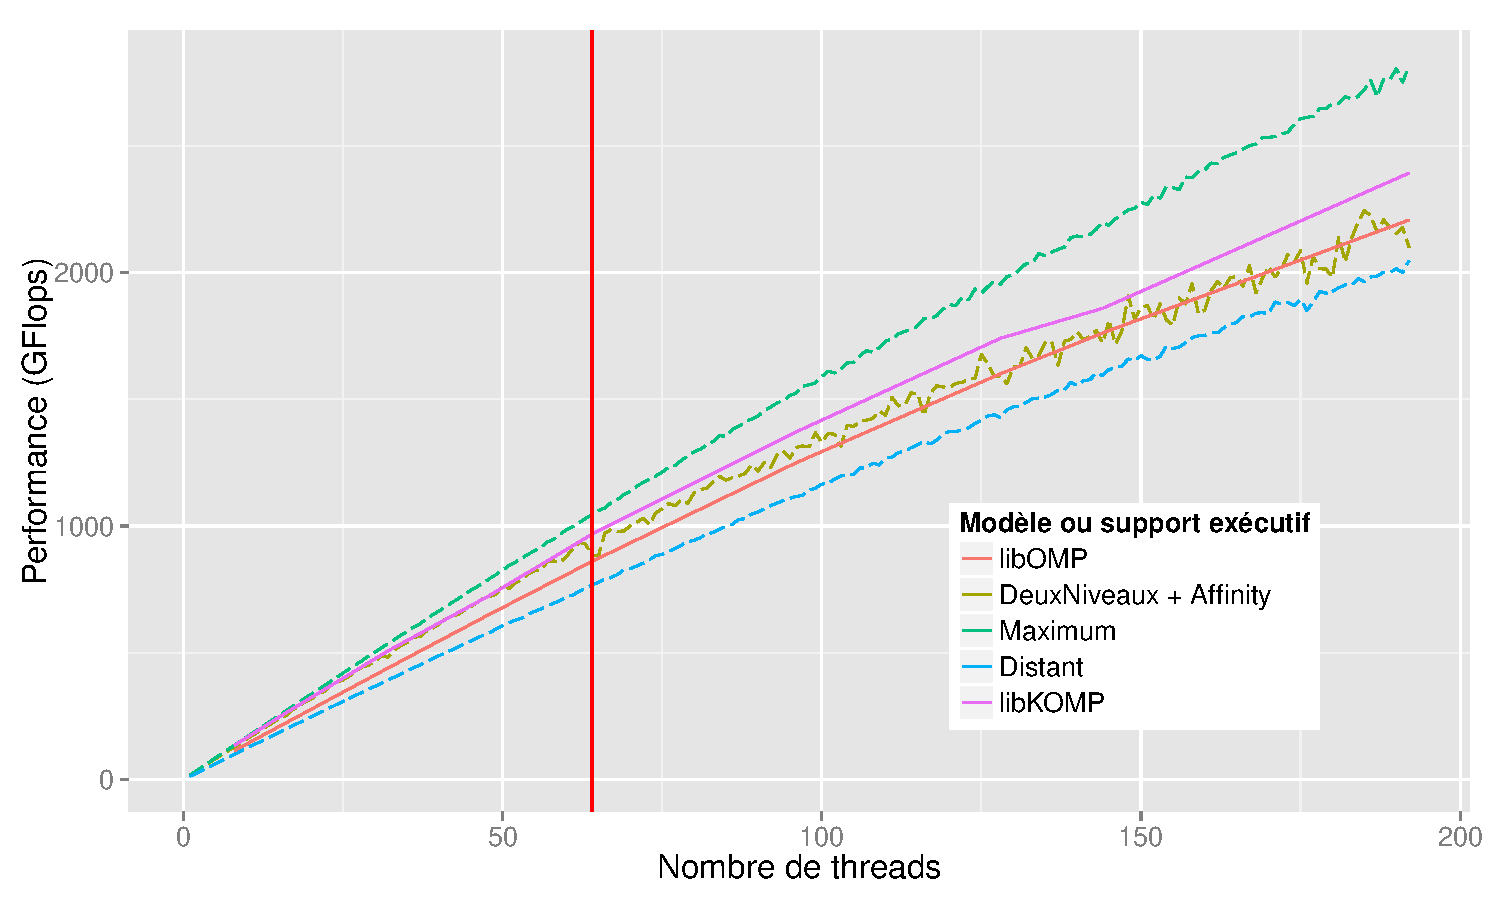
\includegraphics[width=\textwidth]{simu_affinity_runtime_idchire}
  \caption{Comparaison des certains modèles aux supports exécutifs sur idchire, pour une taille de matrice de 32768 et une taille de bloc de 512}\label{fig:simu:modeles-vs-runtime:idchire}
\end{figure}
\begin{figure}[h!]
  \centering
  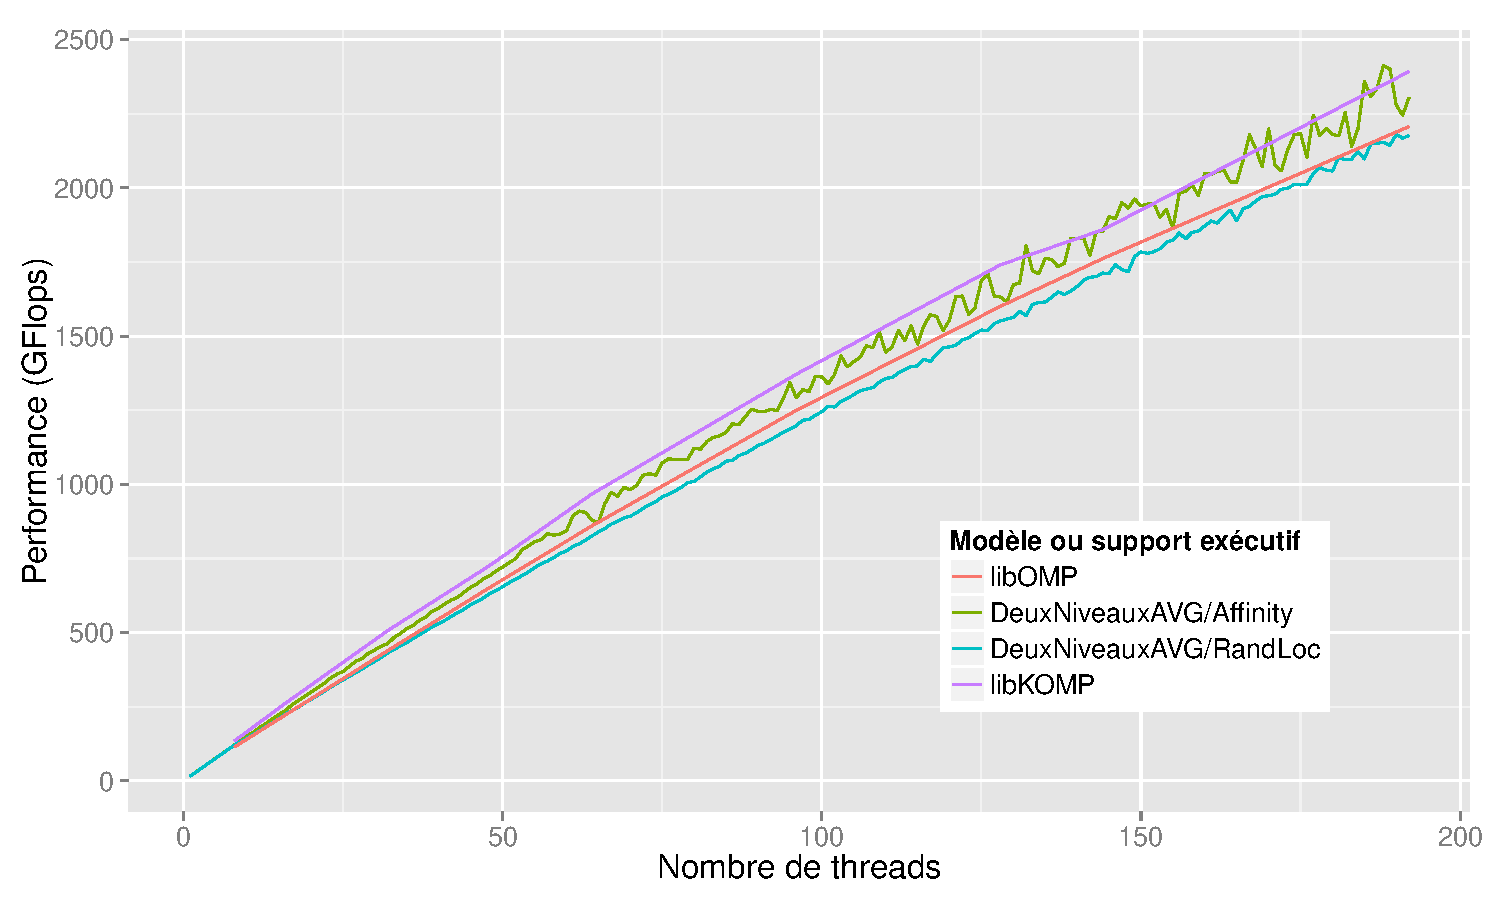
\includegraphics[width=\textwidth]{simu_affinity_avg_runtime_idchire}
  \caption{Comparaison du modèle \emph{AffinityAVG} aux supports exécutifs sur idchire, pour une taille de matrice de 32768 et une taille de bloc de 512}\label{fig:simu:affinityavg-vs-runtime:idchire}
\end{figure}


La figure~\ref{fig:simu:modeles-vs-runtime:idchire} compare les modèles \emph{Minimum} (avec vol aléatoire) et \emph{Affinity} (avec vol hiérarchique) aux supports exécutifs libOMP (qui utilise un vol aléatoire) et libKOMP (qui utilise un vol hiérarchique et l'affinité). libGOMP a été omis pour ne pas surcharger la figure, et parce que son comportement suit celui de libOMP.
Comme on peut le constater, les performances des deux supports exécutifs sont effectivement supérieures au minimum simulé. En revanche les performances simulées de l'affinité semblent faibles compte tenu des performances réelles.

Cette différence pourrait sembler étonnante, mais pourrait être en partie expliquée par le fait que les performances de référence ont été obtenues lorsque les données étaient soit \textit{toutes} locales ou \textit{toutes} distantes.
Alors que dans la réalité il peut évidemment y avoir plusieurs autres cas quand plusieurs blocs sont en paramètre des noyaux.
Cela donnerait donc une version <<minimum>> des performances plus pessimistes que la réalité.

Nous avons essayé de prendre la moyenne globale des performances de chaque noyau comme référence, sous le modèle \emph{AffinityAVG}.
Les résultats obtenus sont présentés sur la figure~\ref{fig:simu:affinityavg-vs-runtime:idchire}.

La simulation des deux heuristiques semblent adhérer un peu mieux à la réalité, bien qu'il semble possible de gagner encore en précision.

Ces travaux étant en cours, plusieurs pistes d'amélioration sont envisagées, et sont décrites dans la section~\ref{sec:simulation:next}.


Les résultats obtenus sur les cas favorable à l'utilisation de l'affinité sont assez encourageants.
Nous avons également appliqué la simulation sur des tailles de bloc plus petites, typiquement pour une taille de matrice de 8192 avec des blocs de 256.

\begin{figure}[h!]
  \centering
  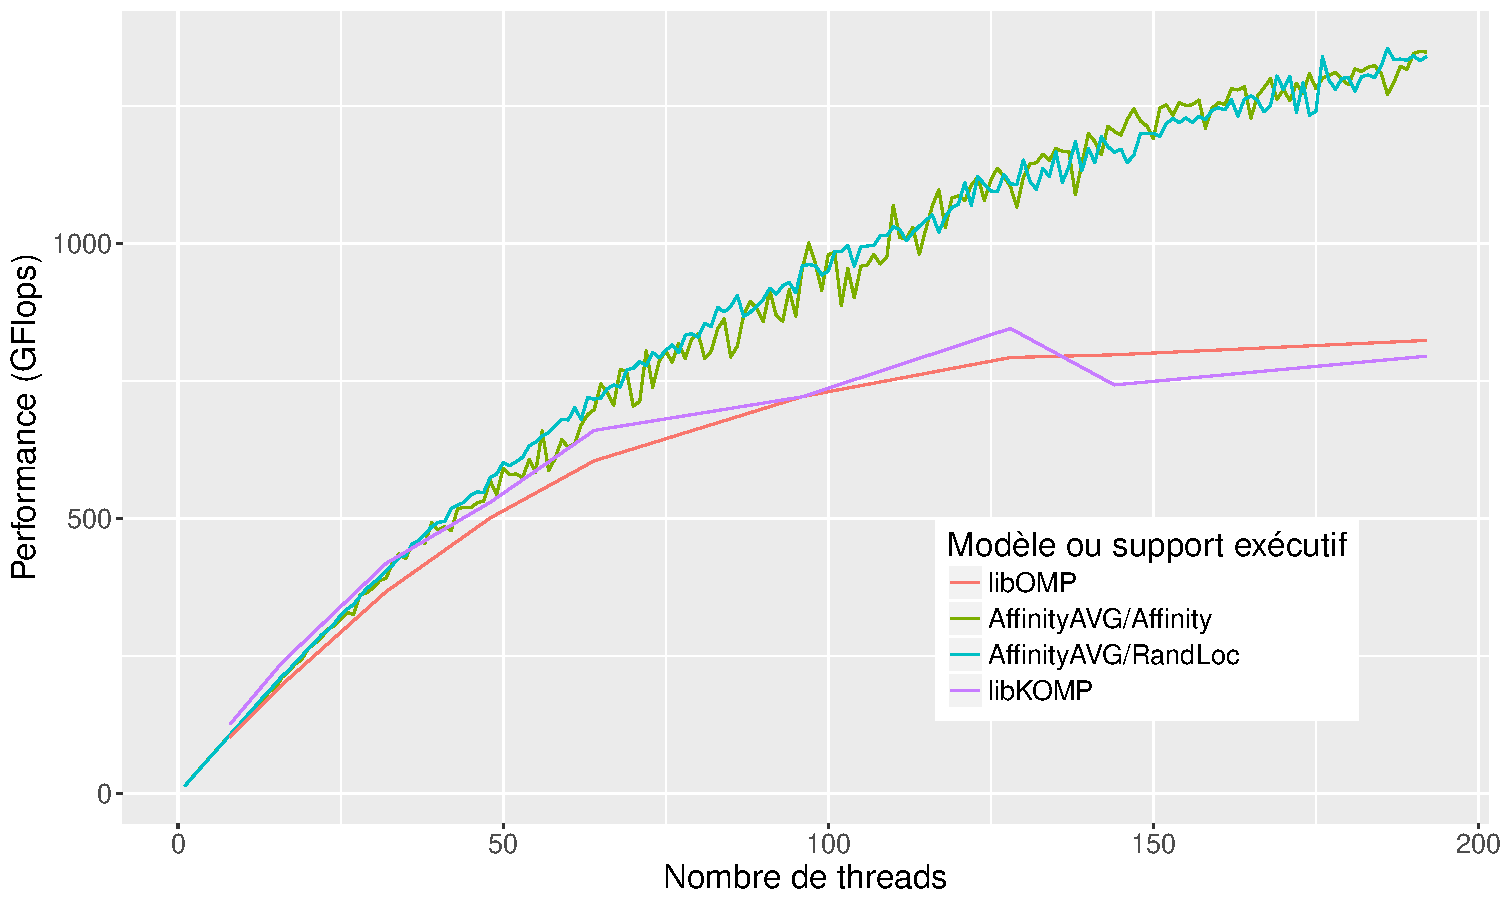
\includegraphics[width=\textwidth]{simu_affinity_8k_runtime_idchire}
  \caption{Comparaison du modèle \emph{AffinityAVG} aux supports exécutifs sur idchire, pour une taille de matrice de 8192 et une taille de bloc de 256}\label{fig:simu:affinityavg-8k-vs-runtime:idchire}
\end{figure}

Les résultats obtenus sont présentés sur la figure~\ref{fig:simu:affinityavg-8k-vs-runtime:idchire}.
Comme on a pu le constater sur les expériences réelles, la simulation ne montre également aucune différence de performances avec ou sans l'utilisation de l'affinité.

En revanche les performances des deux supports exécutifs sont assez loin de celles a priori atteignables !
Le nombre de tâches dans une telle configuration peut vite limiter le parallélisme exposé, ce qui va donc entrainer une augmentation importante du nombre de requêtes de vol émises par les threads inactifs.

\begin{figure}[h!]
  \centering
  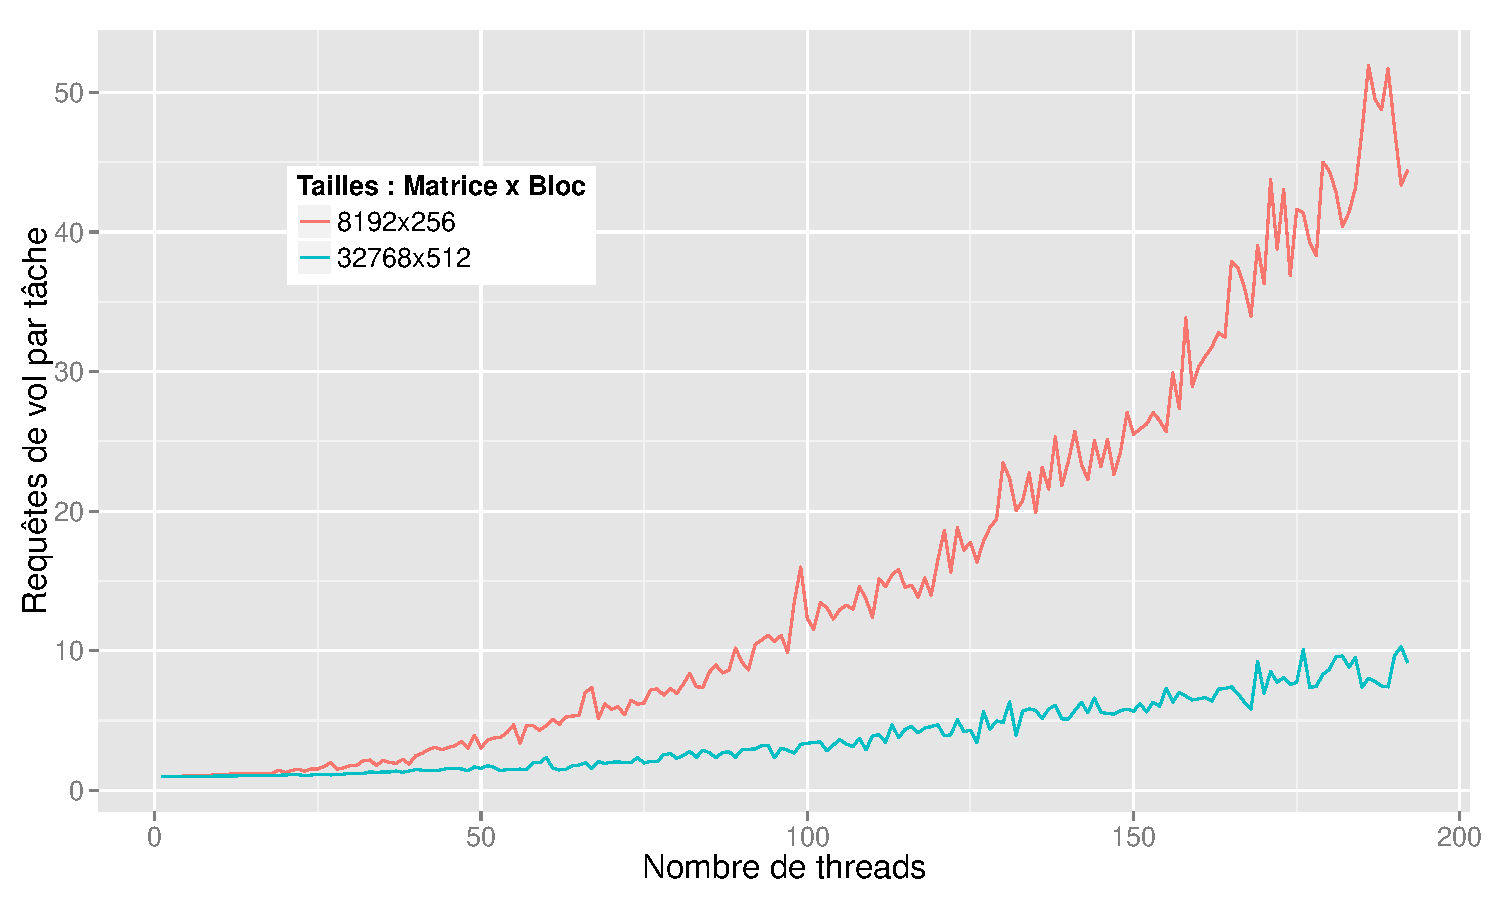
\includegraphics[width=\textwidth]{simu_steal_visits_idchire}
  \caption{Comparaison de l'évolution du nombre de requêtes de vol par tâche dans le simulateur, en fonction de la taille de matrice}\label{fig:simu:steals_per_task:idchire}
\end{figure}

Ce problème est illustré sur la figure~\ref{fig:simu:steals_per_task:idchire}, où l'on voit l'évolution du nombre de requêtes de vol divisé par le nombre de tâches à exécuter.
Pour un cas exposant un fort parallélisme, une taille de matrice de 32768 avec une taille de bloc de 512 et donc plus de 45000 tâches, on peut constater que le nombre de requêtes par tâche reste raisonnable.
En revanche pour le cas étudié dans la figure~\ref{fig:simu:affinityavg-8k-vs-runtime:idchire}, une taille de matrice de 8192 avec une taille de bloc de 256 et donc un peu moins de 6000 tâches, on peut constater que l'évolution du nombre de requêtes de vol par tâche est exponentielle, et qu'il décole un peu après 50 threads, ce qui coïncide avec l'apparition du plateau sur la figure~\ref{fig:simu:affinityavg-8k-vs-runtime:idchire}.

Les requêtes de vol ne sont pas modélisées dans le simulateur, et peuvent générer du trafic sur les bus mémoires~: donc non seulement les threads ne participent plus activement à l'exécution du programme, mais en plus ils peuvent dégrader les performances des threads actifs.
Cela explique en grande partie la différence entre la simulation et la réalité, et pourrait être une piste d'amélioration du modèle.


\section{Application d'un ordonnancement théorique}\label{sec:simulation:theorie}

ref model:

\cite{Pan2014}, Modeling cache coherence misses on multicores

\cite{Stanisic2016}, Fast and Accurate Simulation of Multithreaded Sparse Linear Algebra Solvers

\begin{todo}
GRAPHE : courbes Julien sur Cholesky sélectionnés

+mettre la section dans un endroit approprié, probablement après la description du modèle histoire de dire "ça c'est ce qu'on peut faire au mieux".
\end{todo}

\section{Discussions et améliorations possibles}\label{sec:simulation:next}

Nos travaux sur la simulation sont très récents et encore en cours de développement.
Afin de généraliser la portée du simulateur et améliorer sa précision, nous évoquons ici les différentes pistes en cours d'étude.

\subsection{Modélisation du cache L3}

La version actuelle du simulateur inclu un cache par cœur de taille infinie.
Ce cache est modélisé comme une liste de blocs, dans une \emph{version} particulière.
À chaque écriture du bloc, la version du bloc est incrémentée.
Si une tâche effectue une lecture de ce bloc et que sa version correspond à la version du cache, alors la lecture ne coûte rien, sinon le cout de lecture est demandé au modèle.

Comme indiqué dans les sections précédentes, les modèles envisagés pour l'instant se basent uniquement sur le cout global d'une tâche, plutôt que sur des actions séparées.

L'une des améliorations nécessaires pour augmenter la précision du modèle serait l'introduction d'un cache partagé entre les cœurs d'un même nœud, disposant d'une capacité définie par le modèle, et implémentant une politique d'éviction relativement proche de celle utilisée par le matériel~: \emph{LRU}.

\subsection{Modélisation de la bande passante}

Le chapitre~\ref{chap:contrib:characterization} nous a permis d'étudier en détail le comportement de nos deux machines expérimentales.
Les figures~\ref{fig:contribs:machines:idchire:saturation} et~\ref{fig:contribs:machines:idchire:saturation-output} permettent de conclure par exemple que la bande passante d'idchire se comporte d'une manière assez proche d'un modèle \emph{roofline}, où elle augmente linéairement avant d'atteindre un <<plafond>>.

L'objectif serait donc d'introduire un coût d'accès aux blocs mémoires suivant ce modèle.

\subsection{Modélisation des surcouts d'ordonnancement}

La figure~\ref{fig:simu:affinityavg-8k-vs-runtime:idchire} l'a montré, le simulateur manque d'un moyen de modéliser les coûts liés aux fonctions d'ordonnancement du support exécutif.
Une manière d'aborder cela pourrait être d'associer un très faible coût à chaque requête de vol, et éventuellement de le pondérer par le nombre de threads en train d'effectuer des requêtes, pour modéliser la synchronisation nécessaire.

\subsection{Optimisation de la distribution}

Le simulateur permet d'obtenir des informations précises sur la distribution de données et son impact sur les accès locaux et distants.
Comme on l'a vu dans le tableau~\ref{tab:simu:acces-blocs-idchire}, le vol de travail respectant l'affinité permet de réduire considérablement les accès distants.
Il devrait donc être possible d'utiliser le simulateur pour automatiquement trouver la <<meilleure>> distribution de données (c'est à dire celle qui minimise les accès distants), en se basant sur une distribution cyclique et en introduisant des paramètres tels que le premier nœud considéré, le nombre de blocs alloués en même temps, et le pas lors du parcours des nœuds.
